% \def\bmode{2} % Mode 0 for presentation, mode 1 for a handout with notes, mode 2 fo% r handout without notes
% \if 0\bmode
\documentclass[usenames,dvipsnames,smaller, hyperref={colorlinks=true,urlcolor=magenta,citecolor=cyan,linkcolor=orange}]{beamer}
% \else \if 1\bmode
% \immediate\write18{pdflatex -jobname=\jobname-Handout-Notes\space\jobname}
% \documentclass[usenames,dvipsnames,smaller,handout,hyperref={colorlinks=true,urlcolor=magenta,citecolor=cyan,linkcolor=orange}]{beamer}
% \usepackage{handoutWithNotes}
% \pgfpagesuselayout{2 on 1 with notes}[letterpaper, landscape, border shrink=4mm]
% \else \if 2\bmode
% \immediate\write18{pdflatex -jobname=\jobname-Handout\space\jobname}
% \documentclass[usenames,dvipsnames,smaller,handout,hyperref={colorlinks=true,urlcolor=magenta,citecolor=cyan,linkcolor=orange}]{beamer}
% \fi
% \fi
% \fi

% \documentclass[smaller,handout
% ]{beamer}
%\usepackage{etex}
%\newcommand{\num}{6{} }

% \usetheme[
%   outer/progressbar=foot,
%   outer/numbering=counter,
%  block=fill
% ]{metropolis}

%\useoutertheme{metropolis}

\usetheme{Madrid}
\useoutertheme[subsection=false]{miniframes} % Alternatively: miniframes, infolines, split
\useinnertheme{circles}
\usecolortheme{seahorse}

\usepackage[backend=biber,style=authoryear,maxcitenames=2,maxbibnames=99,safeinputenc,url=false,
eprint=false]{biblatex}
\addbibresource{bib/references.bib}
\AtEveryCitekey{\iffootnote{{\tiny}\tiny}{\tiny}}

%\usepackage{pgfpages}
%\setbeameroption{hide notes} % Only slides
%\setbeameroption{show only notes} % Only notes
%\setbeameroption{hide notes} % Only notes
%\setbeameroption{show notes on second screen=right} % Both

% \usepackage[sfdefault]{Fira Sans}

% \setsansfont[BoldFont={Fira Sans}]{Fira Sans Light}
% \setmonofont{Fira Mono}

%\usepackage{fira}
%\setsansfont{Fira}
%\setmonofont{Fira Mono}
% To give a presentation with the Skim reader (http://skim-app.sourceforge.net) on OSX so
% that you see the notes on your laptop and the slides on the projector, do the following:
% 
% 1. Generate just the presentation (hide notes) and save to slides.pdf
% 2. Generate onlt the notes (show only nodes) and save to notes.pdf
% 3. With Skim open both slides.pdf and notes.pdf
% 4. Click on slides.pdf to bring it to front.
% 5. In Skim, under "View -> Presentation Option -> Synhcronized Noted Document"
%    select notes.pdf.
% 6. Now as you move around in slides.pdf the notes.pdf file will follow you.
% 7. Arrange windows so that notes.pdf is in full screen mode on your laptop
%    and slides.pdf is in presentation mode on the projector.

% Give a slight yellow tint to the notes page
%\setbeamertemplate{note page}{\pagecolor{yellow!5}\insertnote}\usepackage{palatino}


%\usetheme{metropolis}
%\usecolortheme{beaver}
%\usepackage{xcolor}
\definecolor{darkcandyapplered}{HTML}{A40000}
\definecolor{lightcandyapplered}{HTML}{e74c3c}

%\setbeamercolor{title}{fg=darkcandyapplered}
%\setbeamercolor{frametitle}{bg=darkcandyapplered!80!black!90!white}
%\setbeamertemplate{frametitle}{\bf\insertframetitle}
%\setbeamercolor{footnote mark}{fg=darkcandyapplered}
%\setbeamercolor{footnote}{fg=darkcandyapplered!70}
%\Raggedbottom
%\setbeamerfont{page number in head/foot}{size=\tiny}
%\usepackage[tracking]{microtype}


\setbeamertemplate{frametitle}{%
    \nointerlineskip%
    \begin{beamercolorbox}[wd=\paperwidth,ht=2.0ex,dp=0.6ex]{frametitle}
        \hspace*{1ex}\insertframetitle%
    \end{beamercolorbox}%
}



\setbeamerfont{caption}{size=\footnotesize}
\setbeamercolor{caption name}{fg=darkcandyapplered}


%\usepackage[sc,osf]{mathpazo}   % With old-style figures and real smallcaps.
%\linespread{1.025}              % Palatino leads a little more leading

% Euler for math and numbers
%\usepackage[euler-digits,small]{eulervm}
%\AtBeginDocument{\renewcommand{\hbar}{\hslash}}
\usepackage{graphicx,multirow,paralist,booktabs}


%\mode<presentation> { \setbeamercovered{transparent} }

\setbeamertemplate{navigation symbols}{}
\makeatletter
\def\beamerorig@set@color{%
  \pdfliteral{\current@color}%
  \aftergroup\reset@color
}
\def\beamerorig@reset@color{\pdfliteral{\current@color}}
\makeatother

%=== GRAPHICS PATH ===========
\graphicspath{{./images/}}
% Marginpar width
%Marginpar width
%\setlength{\marginparsep}{.02in}


%% Captions
% \usepackage{caption}
% \captionsetup{
%   labelsep=quad,
%   justification=raggedright,
%   labelfont=sc
% }

%AMS-TeX packages

\usepackage{amssymb,amsmath,amsthm} 
\usepackage{bm}
\usepackage{color}

\usepackage{hyperref,enumerate}
\usepackage{minitoc,array}


%https://tex.stackexchange.com/a/31370/2269
\usepackage{mathtools,cancel}

\renewcommand{\CancelColor}{\color{red}} %change cancel color to red

\makeatletter
\let\my@cancelto\cancelto %copy over the original cancelto command
\newcommand<>{\cancelto}[2]{\alt#3{\my@cancelto{#1}{#2}}{\mathrlap{#2}\phantom{\my@cancelto{#1}{#2}}}}
% redefine the cancelto command, using \phantom to assure that the
% result doesn't wiggle up and down with and without the arrow
\makeatother


\definecolor{slblue}{rgb}{0,.3,.62}
\hypersetup{
    colorlinks,%
    citecolor=blue,%
    filecolor=blue,%
    linkcolor=blue,
    urlcolor=slblue
}

%%%TIKZ
\usepackage{tikz}
\usepackage{pgfplots}
\usepackage{pgfplotstable}
\usepackage{pgfgantt}
\usepackage{tikzsymbols}
\pgfplotsset{compat=newest}

\usetikzlibrary{arrows,shapes,positioning,shapes.geometric}
\usetikzlibrary{decorations.markings}
\usetikzlibrary{shadows,automata}
\usetikzlibrary{patterns}
\usetikzlibrary{trees,mindmap,backgrounds}
%\usetikzlibrary{circuits.ee.IEC}
\usetikzlibrary{decorations.text}
% For Sagnac Picture
\usetikzlibrary{%
    decorations.pathreplacing,%
    decorations.pathmorphing%
}
\tikzset{no shadows/.style={general shadow/.style=}}
%
%\usepackage{paralist}


%%% FORMAT PYTHON CODE
%\usepackage{listings}
% Default fixed font does not support bold face
\DeclareFixedFont{\ttb}{T1}{txtt}{bx}{n}{8} % for bold
\DeclareFixedFont{\ttm}{T1}{txtt}{m}{n}{8}  % for normal

% Custom colors
\definecolor{deepblue}{rgb}{0,0,0.5}
\definecolor{deepred}{rgb}{0.6,0,0}
\definecolor{deepgreen}{rgb}{0,0.5,0}

%\usepackage{listings}

% Python style for highlighting
% \newcommand\pythonstyle{\lstset{
% language=Python,
% basicstyle=\footnotesize\ttm,
% otherkeywords={self},             % Add keywords here
% keywordstyle=\footnotesize\ttb\color{deepblue},
% emph={MyClass,__init__},          % Custom highlighting
% emphstyle=\footnotesize\ttb\color{deepred},    % Custom highlighting style
% stringstyle=\color{deepgreen},
% frame=tb,                         % Any extra options here
    % showstringspaces=false            % 
% }}

% % Python environment
% \lstnewenvironment{python}[1][]
% {
% \pythonstyle
% \lstset{#1}
% }
% {}

% % Python for external files
% \newcommand\pythonexternal[2][]{{
% \pythonstyle
% \lstinputlisting[#1]{#2}}}

% Python for inline
% 
% \newcommand\pythoninline[1]{{\pythonstyle\lstinline!#1!}}


\newcommand{\osn}{\oldstylenums}
\newcommand{\dg}{^{\circ}}
\newcommand{\lt}{\left}
\newcommand{\rt}{\right}
\newcommand{\pt}{\phantom}
\newcommand{\tf}{\therefore}
\newcommand{\?}{\stackrel{?}{=}}
\newcommand{\fr}{\frac}
\newcommand{\dfr}{\dfrac}
\newcommand{\ul}{\underline}
\newcommand{\tn}{\tabularnewline}
\newcommand{\nl}{\newline}
\newcommand\relph[1]{\mathrel{\phantom{#1}}}
\newcommand{\cm}{\checkmark}
\newcommand{\ol}{\overline}
\newcommand{\rd}{\color{red}}
\newcommand{\bl}{\color{blue}}
\newcommand{\pl}{\color{purple}}
\newcommand{\og}{\color{orange!90!black}}
\newcommand{\gr}{\color{green!40!black}}
\newcommand{\nin}{\noindent}
\newcommand{\la}{\lambda}
\renewcommand{\th}{\theta}
\newcommand{\al}{\alpha}
\newcommand{\G}{\Gamma}
\newcommand*\circled[1]{\tikz[baseline=(char.base)]{
            \node[shape=circle,draw,thick,inner sep=1pt] (char) {\small #1};}}

\newcommand{\bc}{\begin{compactenum}[\quad--]}
\newcommand{\ec}{\end{compactenum}}

\newcommand{\p}{\partial}
\newcommand{\pd}[2]{\frac{\partial{#1}}{\partial{#2}}}
\newcommand{\dpd}[2]{\dfrac{\partial{#1}}{\partial{#2}}}
\newcommand{\pdd}[2]{\frac{\partial^2{#1}}{\partial{#2}^2}}

\newcommand{\pe}{\pause}

%%%%%%%%%%%%%%%%%%%%%%%%%%%%%%%%%%%%%%%%%%%%%%%%%%%
%%%%%%%%%%%%%%%%%%%%%%%%%%%%%%%%%%%%%%%%%%%%%%%%%%%

\title[CEE 260/MIE 273 2c: Conditional Probability]{{\normalsize CEE 260/MIE 273: Probability and Statistics in Civil Engineering} \\
Lecture M2c: Conditional Probability and Bayes' Theorem}
\date[\today]{\footnotesize \today}
\author{{\bf Prof.\ Oke}}
\institute[UMass Amherst]{
  \begin{tikzpicture}[baseline=(current bounding box.center)]
    \node[anchor=base] at (-7,0) (its) {
\includegraphics[scale=.3]{UMassEngineering_vert}} ;
  \end{tikzpicture}
}



%https://tex.stackexchange.com/questions/55806/mindmap-tikzpicture-in-beamer-reveal-step-by-step
  % \tikzset{
  %   invisible/.style={opacity=0},
  %   visible on/.style={alt={#1{}{invisible}}},
  %   alt/.code args={<#1>#2#3}{%
  %     \alt<#1>{\pgfkeysalso{#2}}{\pgfkeysalso{#3}} % \pgfkeysalso doesn't change the path
  %   },
  % }


\usepackage{listings}

\lstset{language=matlab,
                basicstyle=\scriptsize\ttfamily,
                keywordstyle=\color{blue}\ttfamily,
                stringstyle=\color{blue}\ttfamily,
                commentstyle=\color{gray}\ttfamily,
                morecomment=[l][\color{gray}]{\#}
              }
         
\begin{document}

\maketitle




\begin{frame}
  \frametitle{Outline}
  \tableofcontents
\end{frame}

\begin{frame}
  \frametitle{Recap from Lecture 2b: Theory of Probability}
   \begin{itemize}[<+->]
  \item Three axioms of probability:
    \begin{align*}
      P(E) &\ge 0 \quad \text{and} \quad P(E) \le 1 \\ \pe
      P(S) &= 1 \\ \pe
      P(E_{1}\cup E_{2}\cup \cdots\cup E_{n}) &= P(E_{1}) + P(E_{2}) + \cdots + P(E_{n})~~ \text{(Mutually exclusive)}
    \end{align*}
  \item Addition rule: $P(A\cup B) = P(A) + P(B) - P(AB)$ \pe
  \item Addition rule for mutually exclusive events: $P(A\cup B) = P(A) + P(B)$ (Axiom 3) \pe
  \item Counting \pe
    \begin{itemize}[<+->]
    \item Fundamental principle of counting: number of outcomes for $1, \ldots, k$ events, each with $n_{1},\ldots, n_{k}$ possibilities is $n_{1}\times\cdots \times n_{k}$ \pe
    \item Permutations of $n$ objects: $n! = n(n-1)(n-2)\cdots(2)(1)$ \pe
    \item Permutations (arrangements) of a subset of $k$ items chosen from set of $n$ items: $n!/(n-k)!$ \pe
    \item Combinations (distinct; order not important) of group of $k$ items chosen from set of $n$ items: $n!/(k!(n-k)!)$
    \end{itemize}
  \end{itemize}
\end{frame}
 
\begin{frame}
  \frametitle{Objectives of today's lecture}
  \pause

  \begin{itemize}[<+->]
  \item Understand conditional probability
  \item Grasp the concept of statistical independence
  \item Apply the multiplication rule and understand its relation to conditional probability
  \item Understand total probability
  \item Understand Bayes' Theorem and learn how to apply it to solving inverse probability problems
  \end{itemize}
\end{frame}


  







\section{Conditional probability}
\begin{frame}
  \frametitle{Conditional probability}

  \begin{block}{Definition}
    The probability of an event $E_1$ is  conditional upon another event $E_2$ if the occurrence of $E_1$ is dependent on the occurrence of $E_2$: \pause

    \begin{eqnarray*}
      \label{eq:20}
      P(E_1|E_2) &=& \text{the conditional probability of $E_1$ given $E_2$} \\ \pause
                 && \text{\quad (OR the probability of $E_1$ conditioned on $E_2$)}\\ \pause
      P(E_2|E_1) &=& \pause  \text{the conditional probability of $E_2$ given $E_1$} \\
    \end{eqnarray*}
  \end{block}
\end{frame}

\begin{frame}
  \frametitle{Conditional probability (cont.)}

  We can think of $P(E_1|E_2)$ as the probability of realizing sample points of $E_1$ within the subsample space of $E_2$. \pause
  
  % 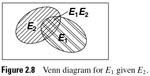
\includegraphics[width=.7\textwidth]{02_08}

    \begin{center}
    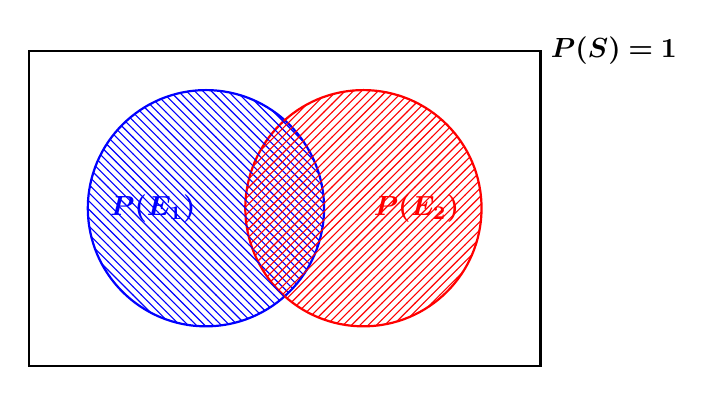
\begin{tikzpicture}[scale=.5]
      \visible<+->{\draw[thick]  (-5,-4) rectangle (8,4) node[anchor=north east, right] {$\bm {P(S) = 1}$};}
      \visible<+->{
        \draw[blue, thick] (-.5,0) circle (3 cm) node[left] {$\bm{P(E_{1})}$};
        \draw[red, thick]  (3.5,0) circle (3 cm) node[right] {$\bm{P(E_{2})}$};
      }
      \visible<+->{
        \fill[pattern=north west lines,pattern color=blue] (-.5,0) circle (3 cm);
      }

      \visible<+->{\fill[pattern=north east lines,pattern color=red](3.5,0) circle (3 cm);
      }
    \end{tikzpicture}      
  \end{center}
  
 
\end{frame}


\begin{frame}
  \frametitle{Conditional probability (cont.)}

  
  % 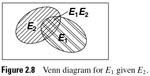
\includegraphics[width=.7\textwidth]{02_08}
 Thus, \pause

  \begin{equation}
    \label{eq:20}
    P(E_1|E_2) = \fr{P(E_1E_2)}{P(E_2)}
  \end{equation}

  \pause
  
    \begin{center}
    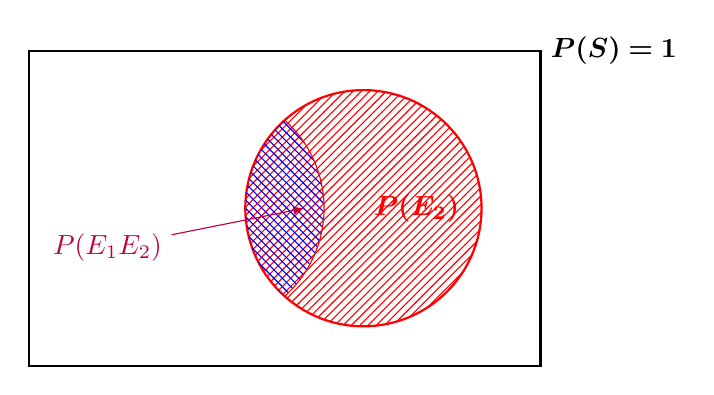
\begin{tikzpicture}[scale=.5]
      \visible<+->{\draw[thick]  (-5,-4) rectangle (8,4) node[anchor=north east, right] {$\bm {P(S) = 1}$};}
      \visible<+->{
        %\draw[blue, thick] (-.5,0) circle (3 cm) node[left] {$\bm{P(E_{1})}$};
        \draw[red, thick]  (3.5,0) circle (3 cm) node[right] {$\bm{P(E_{2})}$};
      }
      \visible<+->{
        \fill[pattern=north east lines,pattern color=red] (3.5,0) circle (3 cm);
      }

      \visible<+->{
        \begin{scope}
          \clip (3.5,0) circle (3 cm);
        \fill[draw,red,pattern=north west lines,pattern color=blue](-.5,0) circle (3 cm);
      \end{scope}
      \node[purple] (A) at (-3,-1) {$P(E_{1}E_{2})$} ;
      \draw[->,>=latex,purple] (A) -- (2,0);
      }
    \end{tikzpicture}      
  \end{center}
  

 
\end{frame}

\begin{frame}
  \frametitle{Useful conditional probability relations}
  \pause
  \begin{eqnarray}
    P(A|S) &=& P(A) \\ \pause
    P(A|B) &=& \fr{P(AB)}{P(B)} \\ \pause
    P(B|A) &=& \fr{P(BA)}{P(A)} = \pause \fr{P(AB)}{P(A)}\\ \pause
    P(\ol{A}|B) &=& 1 - P(A|B)
  \end{eqnarray}

  \pause

  \begin{itemize}[<+->]
  \item A useful mnemonic: think of  ``$|$'' as the division sign.
    \begin{itemize}[<+->]\item 
This means that the event to the right is what goes in the denominator.
\item    The numerator is simply the intersection of both events
  \end{itemize}

  \end{itemize}
\end{frame}

\begin{frame}
  \frametitle{Example 1: Highway routes}\pause

    \begin{minipage}{.45\linewidth}
    There are two routes from City A to City B. One or both routes may be closed due to severe weather. \\ \pause
    We denote $E_1$ as the event Route 1 is open, and $E_2$ as the event Route 2 is open. \\ \pause      
    \end{minipage}\quad
    \begin{minipage}{.45\linewidth}
      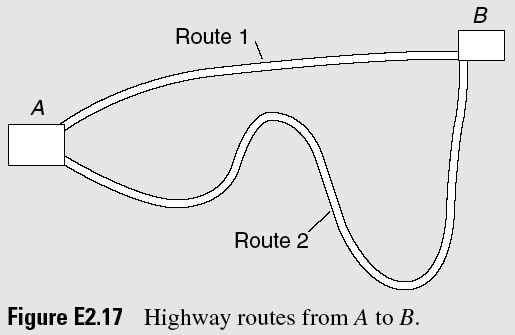
\includegraphics[width=\textwidth, trim={0 1cm 0 0}, clip]{E_02_17}
    \end{minipage}
    \pause
    \medskip
    
    During severe weather, the probabilities the routes will be open are: \pause

    \[ P(E_1) = 0.75 \quad P(E_2) = 0.50 \quad P(E_1E_2) = 0.40 \]
    
    \pause

    \begin{enumerate}[(a)]
    \item What is probability that Route 1 is open during a storm given that Route 2 is also open?
    \item What is probability that Route 2 is open during a storm conditioned on the event that Route 1 is also open?
    \item What is probability that Route 1 is closed during a storm given that Route 2 is also closed?
    \end{enumerate}
\end{frame}



\begin{frame}
  \frametitle{Example 1: Highway routes (cont.)}
    \pause

        \[ P(E_1) = 0.75 \quad P(E_2) = 0.50 \quad P(E_1E_2) = 0.40 \]

        \pause
    \begin{enumerate}[(a)]\gr 
    \item The probability that Route 1 is open ($E_{1}$) during a storm given that Route 2 is also open ($E_{2}$) is denoted as:\pause
      \begin{eqnarray*}
        P(E_1|E_2) &=& \fr{P(E_1E_2)}{P(E_2)} \\ \pause
                   &=& \fr{0.40}{0.50} =  \pause \boxed{0.80}
      \end{eqnarray*}
    \end{enumerate}

  \end{frame}

  \begin{frame}
  \frametitle{Example 1: Highway routes (cont.)}
    \pause

        \[ P(E_1) = 0.75 \quad P(E_2) = 0.50 \quad P(E_1E_2) = 0.40 \]

        \pause
    \begin{enumerate}[(a)]
      \setcounter{enumi}{1} \gr 
    \item The probability that Route 2 is open ($E_{2}$) during a storm conditioned on the event
      that Route 1 is also open ($E_{1}$) is denoted as:\pause
      \begin{eqnarray*}
        P(E_2|E_1) &=& \fr{P(E_2E_1)}{P(E_1)} \\ \pause
                   &=& \fr{0.40}{0.75} =  \pause \boxed{0.53}
      \end{eqnarray*}
    \end{enumerate}

\end{frame}

\begin{frame}
  \frametitle{Example 1: Highway routes (cont.)}\pause

        \[ P(E_1) = 0.75 \quad P(E_2) = 0.50 \quad P(E_1E_2) = 0.40 \]
        \pause
        
    \begin{enumerate}[(a)]
      \setcounter{enumi}{2} \gr 
    \item  The probability that Route 1 is closed ($\ol{E}_{1}$) during a storm given that Route 2 is also closed ($\ol{E}_{2}$) is denoted as:\pause
      \begin{eqnarray*}
        P(\ol{E_1}|\ol{E_2})   &=&  \fr{P(\ol{E_1}\,\ol{E_2})}{P(\ol{E_2})} \\ \pause
        P(\ol{E_1}\,\ol{E_2}) &=& 1 - P(\ol{\ol{E_1}\,\ol{E_2}}) \quad \pause \text{\og complementary events } \\
                              &=& 1 - P(E_1 \cup E_2) \quad \pause \text{\og De Morgan's Rule }\\ \pause
                              &=& 1 - [P(E_1) + P(E_2) - P(E_1E_2)] \quad \pause \text{\og addition rule} \\
                              &=& 1 - (0.75 + 0.50 - 0.40) \\
                              &=& 1 - 0.85 = \pause 0.15
      \end{eqnarray*}
      Thus, we obtain\pause
      \begin{equation*}
        P(\ol{E_1}|\ol{E_2}) = \pause  \fr{P(\ol{E_1}\,\ol{E_2})}{P(\ol{E_2})} = \pause \fr{0.15}{0.50} = \pause  \boxed{0.30}
      \end{equation*}
    \end{enumerate}
 \end{frame}


\begin{frame}
  \frametitle{The addition rule}
  \pause

  Conditioning  equally applies to probabilities of events on the same subsample space. \pause
  \begin{eqnarray}
    \label{eq:17b}
        P(E_1 \cup E_2) &=& P(E_1) + P(E_2) - P(E_1E_2) \\[2mm] \pause
    P(E_1 \cup E_2|A) &=& P(E_1|A) + P(E_2|A) - P(E_1E_2|A)
  \end{eqnarray}
\end{frame}

\section{Independent events}  
\begin{frame}
  \frametitle{Statistically independent events}\pause
  \begin{block}{Statistical independence}\pause
    Two events are statistically independent if the occurence of one does not depend on the occurence or non-occurence of the other:\pause
    \begin{eqnarray}
      P(E_1|E_2) &=& P(E_1) \\ \pause
      P(E_2|E_1) &=& P(E_2)
    \end{eqnarray}
  \end{block}

  \pause

  \begin{exampleblock}{Examples of independent events}\pause
    \begin{itemize}
    \item The outcomes of a die rolled twice in succession. \pause The result of the first roll does not affect the result of the other.
      \pause
    \item The event that it will be cloudy in Amherst tomorrow and the event that the number of births in California tomorrow will increase compared to that of today. \pause (Knowledge of one event cannot improve prediction of the other.) \pause
      
    \item The ages of a random sample of Pioneer Valley residents \pause
      
    \item Generally, all elements of a random sample are assumed independent \pause

    \end{itemize}
  \end{exampleblock}
\end{frame}

\begin{frame}
  \frametitle{Example 2: Rolling two dice}
  \pause

  Let $X$ and $Y$ represent the outcomes of rolling two dice. \pause

  \begin{enumerate}[\bf (a)]
  \item What is the probability that the first die $X$ is 1?\\ \pause
    {\gr    \begin{eqnarray*}
      P(X=1) &=& \fr16
            \end{eqnarray*}
            }
    \pause

    \medskip

  \item What is the probability that both $X$ and $Y$ are 1? \\ \pause

    \medskip
    
    {\gr
    The outcome of $X$ has no bearing on the outcome of $Y$. Thus: \pause
    \begin{eqnarray*}
      P(X =1 \cap Y = 1) &=& P(X=1) \times P(Y=1) \\\pause
                         &=& \fr16 \times \fr16 = \pause \fr1{36}
    \end{eqnarray*}
    }
  \end{enumerate}
\end{frame}

\begin{frame}
  \frametitle{Example 2: Rolling two dice (cont.)}
  \pause

  \begin{enumerate}[\bf (a)]\setcounter{enumi}{2}
  \item Use the conditional probability formula to find $P(Y=1|X=1)$ \\ \pause
   {\gr  \begin{eqnarray*}
      P(Y=1|X=1) &=& \fr{P(Y=1 \cap Y=1)}{P(X=1)} \\ \pause
                 &=& \fr{P(Y=1) \times \cancelto<+->{1}{P(X=1)} }{\cancelto<+->{1}{P(X=1)}} \\\pause
                 &=& P(Y=1)
    \end{eqnarray*}
  }
    \pause

  \item Why is $P(Y=1|X=1) = P(Y=1)$?  \\ \pause

    \medskip
    
    {\gr $X$ and $Y$ are independent events.}
  \end{enumerate}
\end{frame}

\section{Multiplication rule}
\begin{frame}
  \frametitle{The multiplication rule}\pause
  The probability of the intersection of two events is\pause
  \begin{equation}
    \label{eq:13}
    P(E_1E_2) = P(E_1|E_2)P(E_2)
  \end{equation}
  \pause
  \medskip
  
  Equivalently:
  \pause
  \begin{equation}
    \label{eq:14}
    P(E_1E_2) = P(E_2|E_1)P(E_1)
  \end{equation}

  \pause

  \begin{alertblock}{Statistically independent events}
    IF $E_1$ and $E_2$ are statistically independent, the multiplication rule becomes: \pause
    \begin{equation}
      \label{eq:15}
      P(E_1E_2) = P(E_1)P(E_2)
    \end{equation}
    \pause
    That is, the \alert{joint probability} of two statistically independent events is the \alert{product} of their individual probabilities.
  \end{alertblock}
\end{frame}


\begin{frame}
  \frametitle{The multiplication rule: three events}
  The probability of the joint occurrence of three events is:

  \pause

  \begin{align}
    \label{eq:16}
    \notag P(E_1E_2E_3) &= P(E_1|E_2E_3)P(E_2E_3)\\
                 &=  P(E_1|E_2E_3)P(E_2|E_3)P(E_3)
  \end{align}

  \pause
  \begin{alertblock}{Statistically independent events}
    If the three events are statistically independent, then: \pause
    \begin{equation}
      \label{eq:16}
      P(E_1E_2E_3) = \pause P(E_1)P(E_2)P(E_3)
    \end{equation}
  \end{alertblock}
  
\end{frame}


\begin{frame}
  \frametitle{The multiplication rule: conditional probabilities}
  Equally applies to probabilities of events conditioned on the same subsample space. \pause
  \begin{equation}
    \label{eq:17}
    P(E_1E_2|A) = P(E_1|E_2|A)P(E_2|A)
  \end{equation}

  \pause
  \begin{alertblock}{Statistically independent events}
    If $E_1$ and $E_2$ are statistically independent, the multiplication rule for two events conditioned on the same space becomes: \pause
    \begin{equation}
      \label{eq:18}
      P(E_1E_2|A) = P(E_1|A)P(E_2|A)
    \end{equation}
  \end{alertblock}
\end{frame}



\begin{frame}
  \frametitle{Example 3: Airline industry strikes}\pause
  
    The airline industry in a certain country is subject to labor strikes by the
    pilots (event $A$), mechanics (event $B$) or flight attendants (event $C$).\\ \pause

    \bigskip
    
    The probability of strikes by each of the individual groups in the next 3 years is given by:\pause

    \[P(A) = 0.03\quad P(B) = 0.05\quad P(C) = 0.06\]

    \pause 

    Assuming that events $A$, $B$ and $C$ are statistically independent, find

    \begin{enumerate}[\bf (a)]
    \item the probability that all groups will strike in the next 3 years
    \item     the probability of a labor strike in the airline industry in the next 3 years.
    \end{enumerate}

    
\end{frame}


\begin{frame}
  \frametitle{Example 3: Airline industry strikes (cont.)} \pause
  
    \[P(A) = 0.03\quad P(B) = 0.05\quad P(C) = 0.06\]

    \bigskip
    
    {\bf (a) } The probability that all 3 groups will strike in the next 3 years is given by: \pause

    \begin{eqnarray*}
      P(ABC) &=& P(A)P(B)P(C)  \pause \quad \text{\og statistical independence} \\\pause
             &=& 0.03(0.05)(0.06) \\ \pause
             &=& 0.00009 = \pause \boxed{9.0 \times 10^{-5}}
    \end{eqnarray*}
  \end{frame}
  
\begin{frame}
  \frametitle{Example 3: Airline industry strikes (cont.)} \pause
  
    \[P(A) = 0.03\quad P(B) = 0.05\quad P(C) = 0.06\]

    \bigskip

    \pause

    {\bf (b) } The probability of a labor strike is the probability that any combination of the groups will strike. \pause

    
    \begin{enumerate}[(Step 1)]
    \item Formulate the desired probability: \pause
      \begin{equation*}
        P(A\cup B \cup C)
      \end{equation*}
      \pause

    \item Use the complement rule, de Morgan's rule and multiplication rule for statistically independent events: \pause
      \begin{eqnarray*}
        P(A\cup B \cup C) & =& 1 - P(\ol{A\cup B \cup C}) \pause \quad \text{\og complement rule} \\ \pause
                          & =& 1 - P(\ol{A}\,\ol{B}\,\ol{C}) \pause \quad \text{\og de Morgan's rule} \\ \pause
                          & =& 1 - P(\ol{A})P(\ol{B})P(\ol{C}) \pause \quad \text{\og statistical independence} \\\pause
                          &=&  1- (1-0.03)(1-0.05)(1-0.06) \\\pause
        &=& 1 - (0.97)(0.95)(0.94) \\ \pause
        &=& \boxed{0.134}
      \end{eqnarray*}
    \end{enumerate}
    
 \end{frame}



\section{Theorem of total probability}
\begin{frame}
  \frametitle{Total probability}

  Useful in situations where the probability of an event cannot be directly
  determined but its conditional probabilities are known.
  
  \pause
  
  \begin{block}{Theorem of total probability}
    The probability of an event $A$ conditioned on the mutually exclusive and
    collectively exhaustive events $E_1, E_2, \ldots, E_n$ is given by \pause
    \begin{equation}
      \label{eq:19}
      P(A) = P(A|E_1)P(E_1) + P(A|E_2)P(E_2) + \cdots + P(A|E_n)P(E_n)
    \end{equation}
  \end{block}

  \pause

  \begin{minipage}[b]{.55\linewidth}
    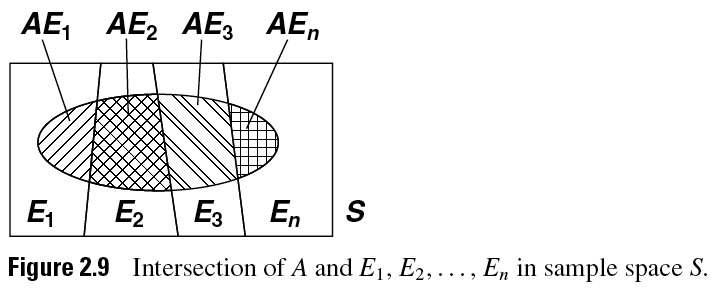
\includegraphics[width=\textwidth,trim={0 1.2cm 11cm 0},clip]{02_09}    
  \end{minipage}\pause\quad
  \begin{minipage}[b]{.4\linewidth}\raggedright
    $P(A)= \pause P(AE_{1}) + \pause P(AE_{2}) $ \pause
    
    \quad\quad\quad $+ \pause P(AE_{3}) + \cdots + P(AE_{n})$  \pause

    \medskip
    
    Note that:\\\pause
    \alert{$P(AE_1) = P(A|E_1)P(E_1)$},\\ etc.
  \end{minipage}
  
\end{frame}


\begin{frame}
  \frametitle{Example 4: Flooding and snow accumulation}\pause
    The flooding of a river in the spring season (event $F$) will depend on the
    accumulation of snow in the mountain during the past winter.\pause The
    accumulation of snow may be heavy ($H$), normal ($N$) or light ($L$).\\ \pause

    \bigskip
    
    Given: \pause
    \[ P(F|H) = 0.90\quad P(F|N) = 0.40 \quad P(F|L) = 0.10 \]
    and in the winter\pause
    \[P(H) = 0.20\quad P(N) = 0.50\quad P(L) = 0.30 \]
    \pause

    Find the probability of flooding in the river during the spring season $P(F)$.
 \end{frame}


\begin{frame}
  \frametitle{Example 4: Flooding and snow accumulation (cont.)} \pause
    We use the theorem of total probability: \pause

    \begin{eqnarray*}
      P(F) &=& P(F|H)P(H) + P(F|N)P(N) + P(F|L)P(L) \\ \pause
           &=& 0.90(0.20) + 0.40(0.50) + 0.10(0.30) \\ \pause
           &=& 0.41
    \end{eqnarray*}
 \end{frame}
    
\section{Bayes' theorem}
\begin{frame}
  \frametitle{Derivation of Bayes' theorem} \pause
  
  Recall from the multiplication rule that:\pause
  \begin{equation}
    \label{eq:21}
    P(AB) =   \rd P(A|B)P(B)
  \end{equation}

  \pause

  \medskip
  
  Equivalently: \pause
  \begin{equation}
    \label{eq:22}
    P(AB) =\bl P(B|A)P(A) 
  \end{equation}
  \pause

  We combine both equations to obtain:
  \pause
  \begin{equation}
    \label{eq:23}
   {\rd P(A|B)P(B)} = {\bl P(B|A)P(A)}
  \end{equation}

  \pause

  \medskip
  
  Then, we obtain the \textbf{inverse probability} of the conditioning event:\pause
  \begin{equation}
    \label{eq:24}
    P(B|A) = \fr{P(A|B)P(B)}{P(A)}
  \end{equation}
  \pause

  This is in essence Bayes' Theorem
\end{frame}


\begin{frame}
  \frametitle{Bayes' theorem}\pause

  Bayes' Theorem allows for the computation of an inverse probability, e.g. given $P(A|B)$, can we find $P(B|A)$?
  
  \pause
  \begin{block}{}
    \begin{minipage}{.75\linewidth}
       
  \begin{equation}
    \label{eq:25}
    {\pl P(E_i|A)} =\fr{P(A|E_i)P(E_i)}{\sum_{j=1}^{n}P(A|E_j)P(E_j)} = \pause \fr{{\rd P(A|E_i)}{\bl P(E_{i})}}{\gr P(A)}
  \end{equation}
  \vspace{-3ex}
  \pause
  \begin{itemize}[<+->]
  \item {\bf posterior probability: $\pl P(E_i|A)$}
  \item {\bf likelihood: $\rd P(A|E_{i}$}
  \item {\bf prior: $\bl P(E_{i})$}
  \item {\bf evidence (total probability): $\gr P(A)$}
  \end{itemize}   
    \end{minipage}\quad
    \begin{minipage}{.2\linewidth}
      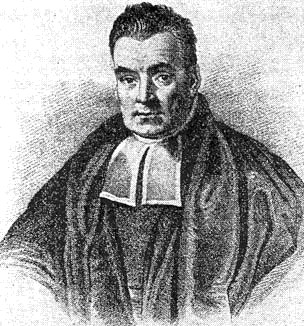
\includegraphics[width=.6\linewidth]{Bayes.png}

      \footnotesize  Rev.\ Thomas Bayes\\
      (1701-61)
    \end{minipage}
    
\end{block}

\pause

If the event $A$ can be conditioned on only two events $E_{1}$ and $E_{2}$, then: \pause

\begin{eqnarray}
  P(E_{1}|A) &=& \pause \fr{P(A|E_{1})P(E_{1})}{P(A|E_{1})P(E_{1}) + P(A|E_{2})P(E_{2}) } \\[2mm] \pause
  P(E_{2}|A) &=& \pause \fr{P(A|E_{2})P(E_{2})}{P(A|E_{1})P(E_{1}) + P(A|E_{2})P(E_{2}) } 
\end{eqnarray}
\end{frame}


\begin{frame}
  \frametitle{Example 5: Construction supplies}
    Aggregates for the construction of a reinforced concrete building are supplied by two companies. \pause
    Company $a$ delivers 600 truckloads a day while Company $b$ delivers 400 truckloads a day. \pause
    From prior experience, 3\% of Company $a$'s material is expected to be substandard while 1\% of Company $b$'s material is expected to be susbstandard.\\ \pause

    We define: \pause

    \begin{eqnarray*}
      A &=& \text{aggregates supplied by Company $a$} \\\pause
      B &=& \text{aggregates supplied by Company $b$} \\\pause
      E &=& \text{aggregates are substandard} 
    \end{eqnarray*}
 
\end{frame}


\begin{frame}
  \frametitle{Example 5: Construction supplies (cont.)}
  \pause
  
  \begin{enumerate}[(a)]
  \item Draw a Venn diagram and convince yourself that $P(A) = 0.60, P(B) = 0.40, P(E|A) = 0.03, P(E|B) = 0.01$ \pause

    \bigskip
    
    \begin{center}
      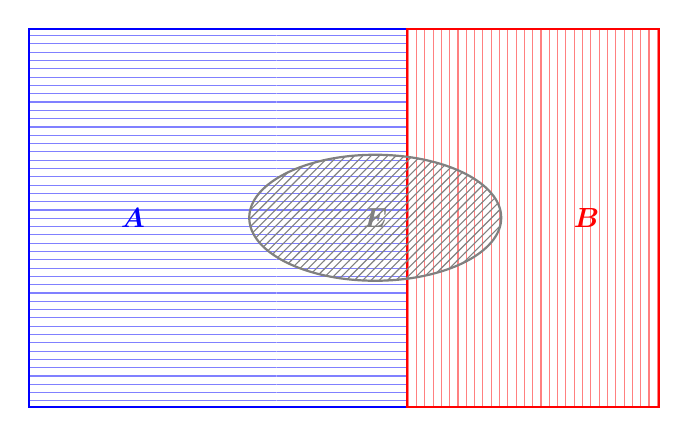
\begin{tikzpicture}[scale=.8]
        \visible<+->{
          \draw[thick,blue, pattern=horizontal lines, pattern color=blue!50!]  (0, 0) rectangle (6,6);
          \node[blue,left] at (2,3) {$\bm A$};
        } % node[anchor=north east, right] {$\bm S$};}
        \visible<+->{
          \draw[thick, red, pattern=vertical lines, pattern color=red!50!]  (6, 0) rectangle (10,6);
          \node[red,right] at (8.5,3) {$\bm B$};
        } 
        \visible<+->{
          \draw[thick,gray, pattern=north east lines, pattern color=gray] (5.5,3) ellipse (2 cm and 1 cm) node[gray] {$\bm E$};
        }

      \end{tikzpicture}
    \end{center}  
    
  \end{enumerate}
\end{frame}

\begin{frame}
  \frametitle{Example 5: Construction supplies (cont.)}\pause

  \[P(A) = 0.60, P(B) = 0.40, P(E|A) = 0.03, P(E|B) = 0.01\]\pause
  
  \begin{enumerate}[(a)]
  \item $P(E|A) = \frac{P(EA)}{P(A)}$
    \pause
    \begin{center}
      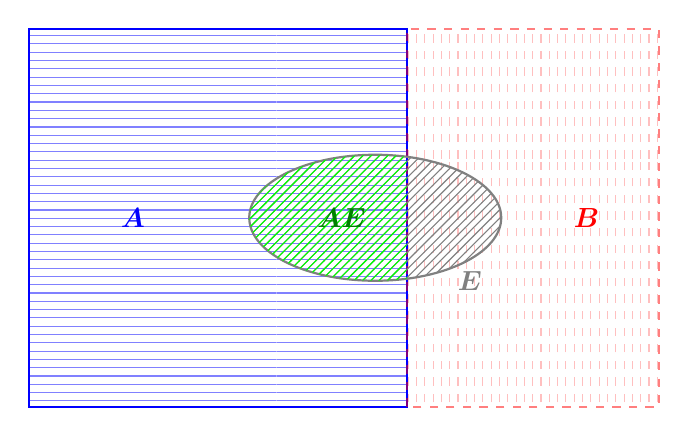
\begin{tikzpicture}[scale=.8]
        \visible<+->{
          \draw[thick,blue, pattern=horizontal lines, pattern color=blue!50!]  (0, 0) rectangle (6,6);
          \node[blue,left] at (2,3) {$\bm A$};
        } % node[anchor=north east, right] {$\bm S$};}
        \visible<+->{
          \draw[dashed,opacity=.5,thick, red, pattern=vertical lines, pattern color=red!50!]  (6, 0) rectangle (10,6);
          \node[red,right] at (8.5,3) {$\bm B$};
        } 
        \visible<+->{
          \draw[gray,thick, pattern=north east lines, pattern color=gray] (5.5,3) ellipse (2 cm and 1 cm);
          \node[gray] at (7,2) {$\bm E$};
        }
        
        % \visible<8->{
        % \fill[white] (-1,0) ellipse (3 cm and 1 cm) ;
        % \fill[white] (3,0) ellipse (4 cm and 1 cm) ;
        % \fill[draw,pattern=north east lines,pattern color=green!50!black]
        % (-1,0) ellipse (3 cm and 1 cm) node[left] {$\bm{P(E_{1})}$};
        % }
        
          \visible<+->{        
          \begin{scope}%[even odd rule]
            \clip (0, 0) rectangle (6,6);
            \fill[green,pattern=north east lines, pattern color=green] (5.5,3) ellipse (2 cm and 1 cm) node[green!50!black,left]
            {$\bm {AE}$};
           % \node at (4,0)  {$\bm{P(E_{2}) -  P(E_{1}E_{2})}$};
          \end{scope}
          %\draw[] (-1,0) ellipse (3 cm and 1 cm) ;
          %\draw[]  (3,0) ellipse (4 cm and 1 cm);
        }

      \end{tikzpicture}
    \end{center}
  \end{enumerate}
\end{frame}


\begin{frame}
  \frametitle{Example 5: Construction supplies (cont.)}\pause

  \[P(A) = 0.60, P(B) = 0.40, P(E|A) = 0.03, P(E|B) = 0.01\]\pause
  
  \begin{enumerate}[(a)]
  \item $P(E|B) = \frac{P(EB)}{P(B)}$
    \pause
    \begin{center}
      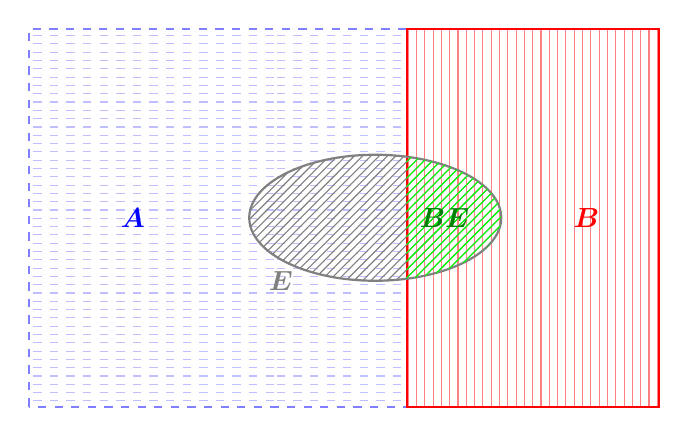
\begin{tikzpicture}[scale=.8]
        \visible<+->{
          \draw[dashed,opacity=.5,thick,blue, pattern=horizontal lines, pattern color=blue!50!]  (0, 0) rectangle (6,6);
          \node[blue,left] at (2,3) {$\bm A$};
        } % node[anchor=north east, right] {$\bm S$};}
        \visible<+->{
          \draw[thick, red, pattern=vertical lines, pattern color=red!50!]  (6, 0) rectangle (10,6);
          \node[red,right] at (8.5,3) {$\bm B$};
        } 
        \visible<+->{
          \draw[gray,thick, pattern=north east lines, pattern color=gray] (5.5,3) ellipse (2 cm and 1 cm);
          \node[gray] at (4,2) {$\bm E$};
        }
        \visible<+->{        
          \begin{scope}%[even odd rule]
            \clip (6, 0) rectangle (10,6);
            \fill[green,pattern=north east lines, pattern color=green] (5.5,3) ellipse (2 cm and 1 cm);
            \node[green!50!black] at (6.6,3)  {$\bm {BE}$};
          \end{scope}
        }

      \end{tikzpicture}
    \end{center}
  \end{enumerate}
\end{frame}


\begin{frame}
  \frametitle{Example 5: Construction supplies (cont.)}

  \[P(A) = 0.60, P(B) = 0.40, P(E|A) = 0.03, P(E|B) = 0.01\]\pause

    \begin{enumerate}[(a)]\setcounter{enumi}{1}
     \item Show that $P(E) = 0.022$ \pause

       \bigskip
       
       We use the Theorem of Total Probability:
       {\gr
       \begin{eqnarray*}
         P(E) &=& P(E|A)P(A) + \pause P(E|B)P(B) \\ \pause
              &=& (0.03)(0.6) + \pause (0.01)(0.4) \\ \pause
              &=& 0.018 + \pause 0.004 \\ \pause
              &=& \boxed{0.022}
       \end{eqnarray*}
     }
     
     \end{enumerate}
 \end{frame}

 % \begin{frame}
 %  \frametitle{Example 2: Construction supplies (cont.)}

 %  \[P(A) = 0.60, P(B) = 0.40, P(E|A) = 0.03, P(E|B) = 0.01\]\pause

 %    \begin{enumerate}[(a)]\setcounter{enumi}{1}
 %     \item Show that $P(E) = 0.022$ \pause

 %       \bigskip
       
 %       Alternately, we can use a tree diagram

       
 %     \end{enumerate}
 %   \end{frame}

   
\begin{frame}
  \frametitle{Example 5: Construction supplies (cont.)}

    \begin{enumerate}[(a)]\setcounter{enumi}{2}
    \item Show that the probability $P(A|E) = 0.82$ and discuss its significance

      \bigskip

      Here, we use Bayes' Theorem: \pause

      \begin{eqnarray*}
        P(A|E) &=& \fr{\bl P(E|A)P(A)}{{\bl P(E|A)P(A)} + P(E|B)P(B)} \\\pause
               &=& \fr{P(E|A)P(A)}{P(E)} \quad \text{Denominator: total probability} \\ \pause
               &=& \fr{{\bl 0.03} \times {\rd 0.60}}{\gr 0.022} \pause \equiv 
                   \fr{ {\bl \text{likelihood}} \times \text{\rd prior}}{\gr \text{evidence}} \\ \pause
               &=& 0.818 \approx \boxed{0.82}
      \end{eqnarray*}
      \pause

      $P(A|E)$ is the posterior probability of $A$ having observed $E$. In other words, having prior knowledge of $A$ (i.e. $P(A)$ and the likelihood of of $E$ given $A$, we can update our knowledge of $A$ (posterior probability) based on these observations.
    \end{enumerate}
 \end{frame}


 


\section{Outlook}
\begin{frame}
  \frametitle{Recap}
  \begin{itemize}[<+->]
  \item \textbf{Conditional probability}:\pause
    \begin{equation}
      P(A|B) = \fr{P(AB)}{P(B)}
    \end{equation}
    \pause
    
  \item \textbf{Independent events}:\pause
    \begin{equation}
      P(AB) = P(A)P(B)
    \end{equation}
    \pause
    Generally, the joint probability (intersection) of any number of independent events is the product of their individual probabilities:
    \pause
    \begin{equation}
      P(E_{1}\cap E_{2}\cap \cdots \cap E_{n}) = P(E_{1})P(E_{2})\cdots P(E_{n})
    \end{equation}\pause
  \item \textbf{Multiplication rule}:\pause
    \begin{equation}
      P(AB) = P(A|B)P(B) = P(B|A)P(A)
    \end{equation}
  \end{itemize}
\end{frame}
 

\begin{frame}
  \frametitle{Recap (cont.)}
  \begin{itemize}[<+->]
  \item Total probability:
    \begin{equation}
      P(A) = P(A|E_{1})P(E_{1}) + P(A|E_{2})P(E_{2}) + \cdots + P(A|E_{n})P(E_{n})
    \end{equation}

  \item Bayes' Theorem:
    \begin{equation}
      P(E_{1}|A) = \fr{P(A|E_{1})P(E_{1})}{ P(A|E_{1})P(E_{1}) + P(A|E_{2})P(E_{2}) + \cdots + P(A|E_{n})P(E_{n})}
    \end{equation}

  \end{itemize}
\end{frame}

%\backupbegin
\section{Appendix}


%\backupend

%\begin{frame}[allowframebreaks]
%   \frametitle{References}
%   \AtNextBibliography{\scriptsize}
%   \setbeamertemplate{bibliography item}[text]
%   \printbibliography[heading=none]
  
% \end{frame}

%\printbibliography
\end{document}
%%% Local Variables:
%%% mode: latex
%%% TeX-master: t
%%% End:
